\documentclass{../zirkelblatt}
\usepackage{young}
\usepackage{geometry}
\geometry{tmargin=2cm,bmargin=3cm,lmargin=3cm,rmargin=3cm}
\usepackage{float}
\floatstyle{ruled}
\restylefloat{figure}
\newcommand{\head}[1]{\section*{\rmfamily #1}}%begin{center}\large \textbf{#1}\end{center}}
\let\raggedsection\centering
\newcommand{\fuzzy}{\mathrel{||}}
\newcommand{\ol}[1]{\ensuremath{\overline{#1}}}
\newcommand{\ZZ}{\mathbb{Z}}
\newcommand{\RR}{\mathbb{R}}

\begin{document}

\maketitle{Klasse 11./12., Gruppe 2}{3. Mai 2014: \\ Elliptische Kurven}

Das Prototypbeispiel einer \emph{elliptischen Kurve} ist die Menge der
Lösungen~$(x|y)$ der folgenden Gleichung. In den vier Grafiken unten ist die
Kurve abgebildet.
\[ y^2 = x^3 - x - 1. \]
Andere elliptische Kurven erhält man, wenn man an den Zahlenwerten dreht.

\begin{aufgabeShaded}{Etwas Kurvendiskussion}
\begin{enumerate}
\item Wieso ist der Graph zur~$x$-Achse symmetrisch?
\item Wieso gibt es, wenn man genügend weit nach links geht, keine Punkte der
Kurve?
\item Kannst du eine Gleichung für die (gekrümmten) Asymptoten finden?
\end{enumerate}
\end{aufgabeShaded}

\textbf{Das Besondere an elliptischen Kurven} ist folgende bemerkenswerte Tatsache:
\begin{quote}
Jede Gerade durch zwei Punkte einer elliptischen Kurve schneidet die Kurve in
\emph{genau einem weiteren Punkt} -- wenn man richtig zählt.
\end{quote}
\begin{figure}[b]
  \centering
  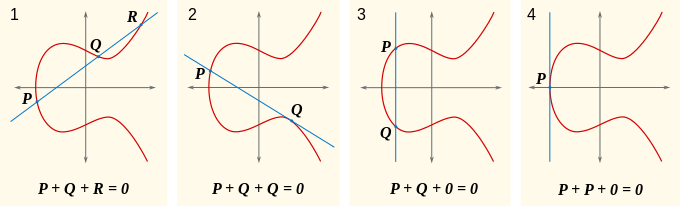
\includegraphics[scale=0.6]{elliptic-curve-r}
  \caption{Vier Schnittsituationen bei der elliptischen Kurve~$y^2 = x^3 - x - 1$}
\end{figure}
Die Abbildung unten demonstriert diesen Sachverhalt.
\begin{itemize}
\item Der einfachste Fall liegt
in Grafik~1 vor: Die Gerade durch die Kurvenpunkte~$P$ und~$Q$ schneidet die
Kurve offensichtlich in genau einem weiteren Punkt, nämlich~$R$.
\item Bei Grafik~2
ist die Situation nicht ganz so offensichtlich: Die Gerade durch die dortigen
Punkte~$P$ und~$Q$ schneidet die Kurve in keinem weiteren Punkt. Allerdings
schneidet die Gerade die Kurve bei~$Q$ nicht nur, sondern \emph{berührt} sie
sogar. Berührpunkte wollen wir doppelt zählen; dann passt die Regel wieder: Die
insgesamt drei Schnittpunkte sind~$P$, $Q$ und~$Q$.
\item In Grafik~3 sind ebenfalls keine weiteren Schnittpunkte zu sehen. Aber
hier haben wir keine Rechtfertigung, einen der Punkte doppelt zu zählen: Unsere
Berührpunktregel greift nicht, und daher wäre es völlig willkürlich, einen der
beiden Punkte doppelt zu werten. Stattdessen sagen wir hier,
dass der dritte Schnittpunkt ein gewisser \emph{Punkt im Unendlichen} ist (dazu
gleich ein Exkurs).
Diesen schreiben wir -- vielleicht etwas seltsamerweise -- als Null (statt
als~$\infty$).
\item Der Sonderfall in Grafik~4 ist eine Kombination aus den beiden vorherigen
Spezialfällen: Der Schnittpunkt~$P$ ist sogar ein Berührpunkt; die insgesamt
drei Schnittpunkte sind daher~$P$,~$P$ und~$0$.
\end{itemize}

\textbf{Exkurs zu Punkten im Unendlichen.} Die gewöhnliche zweidimensionale
Ebene hat einen Schönheitsfehler: Die Merkregel "`je zwei Geraden schneiden
sich"' stimmt nicht uneingeschränkt -- denn bekanntlich schneiden sich
parallele Geraden nicht. Dieses Manko behebt die zweidimensionale
\emph{projektive Ebene}. Diese erklärt man oft über eine Analogie mit
perspektivischer Darstellung: Zwei parallele Bahnschienen schneiden sich nicht
in der gewöhnlichen Ebene. Ihre Abbilder in einer perspektivischen Zeichnung
schneiden sich aber durchaus, im Fluchtpunkt.

Auf der elliptischen Kurve liegt genau ein solcher Punkt im Unendlichen;
anschaulich befindet er sich sowohl "`ganz oben"' als auch "`ganz unten"' auf
jeder Parallelen zur~$y$-Achse.


\head{Gruppenstruktur}

Dank der besonderen Schnitteigenschaft kann man eine
\emph{Gruppenstruktur} auf der Menge der Punkte einer elliptischen Kurve definieren.
Das ist eine Rechenoperation "`Punkt plus Punkt gibt Punkt"'. Wie die
gewöhnliche Addition von Zahlen notiert man diese mit dem Plus-Symbol, und wie
bei der gewöhnliche Addition gelten Eigenschaften wie
\[ P + 0 = P, \qquad P + Q = Q + P, \qquad (P + Q) + R = P + (Q + R). \]
Sonst hat diese neue Rechenoperation aber wenig mit der bekannten Addition zu
tun. Auch die Vektoraddition ist hierfür nur indirekt relevant.

\begin{quote}Immer, wenn Kurvenpunkte~$P, Q, R$ auf einer gemeinsamen Geraden
liegen, definieren wir~$P + Q + R = 0$.
\end{quote}

\begin{aufgabeShaded}{Erste Rechnungen mit Kurvenpunkten}
\begin{enumerate}
\item Was ist das Negative~$-P$ eines Punkts~$P$? Gib dazu eine Vermutung ab
und zeige dann, dass die Probe aufgeht -- zeige also, dass die Gleichung~$P +
\text{Vermutung} + 0 = 0$ stimmt.
\item Seien~$P$ und~$Q$ Kurvenpunkte. Sei~$R$ der eindeutig bestimmte weitere
Kurvenpunkt, der auf der Geraden durch~$P$ und~$Q$ liegt. Mache dir klar, dass
dann~$P + Q$ die Spiegelung von~$R$ an der~$x$-Achse ist.
\item Rechne mit der Beschreibung aus Teilaufgabe~b) nach, dass der Punkt im
Unendlichen das \emph{neutrale Element} der Gruppe ist: Rechne also nach, dass
für jeden Punkt~$P$ die Rechnung~$P + 0 = P$ gilt.
\item Studiere die Animation auf
\url{http://upload.wikimedia.org/wikipedia/commons/7/7e/EllipticGroup.gif}, um
einen Eindruck des Assoziativgesetzes zu erhalten.
\end{enumerate}
\end{aufgabeShaded}

\begin{figure}[t]
  \centering
  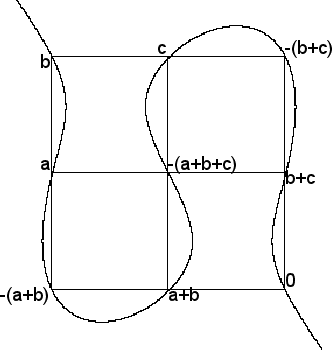
\includegraphics[scale=0.4]{elliptic-curve-associativity}
  \caption{Ein Ausschnitt aus der Animation zur Assoziativitätsdemonstration}
\end{figure}

Mit Teilaufgabe~b) kann man also die Summe von Kurvenpunkten explizit
bestimmen. Ferner können wir eine Rechenoperation "`natürliche Zahl mal Punkt
gibt Punkt"' definieren -- und zwar genau so, wie man auch die gewöhnliche
Multiplikation von Zahlen auf die Addition von Zahlen zurückführt:
\[ n P := \underbrace{P + P + \cdots + P + P}_{\text{$n$ Summanden}}. \]
Ganz konkret ist~$2 P = P + P$ und~$3 P = P + P + P$.

\begin{aufgabeShaded}{Effiziente Multiplikation}
\begin{enumerate}
\item Berechne als Aufwärmübung zeichnerisch für einen Kurvenpunkt~$P$ deiner Wahl die
Punkte~$2P$ und~$3P$.
\item Um den Punkt~$16P$ zu berechnen, müsste man eigentlich fünfzehn Addition
durchführen. Das macht keinen Spaß. Kannst du ein effizienteres Verfahren
finden, das mit nur vier Additionen auskommt?
\item Wie kann man~$1000P$ effizient berechnen?
\end{enumerate}
\end{aufgabeShaded}

Es ist also \emph{leicht}, große Multiplikationen~$nP$ auszuführen. Die
Umkehrung ist aber \emph{schwierig}: Wenn Punkte~$P$ und~$Q$ gegeben sind, und
man gesagt bekommt, dass für irgendeine natürliche Zahl~$n$ die Gleichung~$Q =
nP$ gilt, hat man große Mühe, die Zahl~$n$ zu bestimmen. Man kann natürlich
durchprobieren: Stimmt es für~$n = 1$? Für~$n = 2$? Für~$n = 3$? Und so weiter.
Aber es ist kein Verfahren öffentlich bekannt, dass irgendwie clever abkürzen
könnte. Man vermutet auch, dass es ein solches Verfahren nicht geben kann; das
hat man aber noch nicht beweisen können.


\head{Anwendungen in der Kryptographie}

Manche der kryptographischen Verfahren, die wir kennengelernt haben, haben den
Restklassenring~$\ZZ/(n)$ verwendet. Solche Verfahren kann man oftmals so
umformulieren, dass sie stattdessen die Gruppenstruktur auf einer elliptischen
Kurve verwenden. Ein Vorteil unter weiteren ist, dass man \emph{bei kürzeren
Schlüssellängen gleiche Sicherheit} erzielen kann.

\begin{figure}[b!]
  \centering
  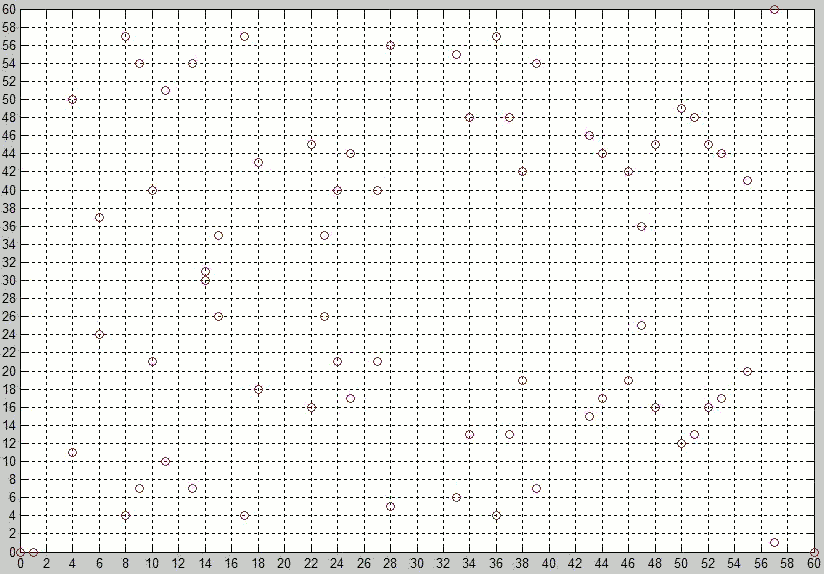
\includegraphics[scale=0.4]{elliptic-curve-z61}
  \caption{Die elliptische Kurve~$y^2 = x^3 - x$ über dem endlichen
  Körper~$\ZZ/(61)$}
\end{figure}

Bei diesen Anwendungen verwendet man keine elliptischen Kurven über~$\RR$,
sondern solche über \emph{endlichen Körpern}. Ein solcher ist etwa der
Restklassenring~$\ZZ/(2)$, der genau zwei Elemente enthält; für jede
Primzahlpotenz~$p^n$ gibt es einen Körper, der~$p^n$ viele
Elemente enthält. (Vorsicht, Falle: Der Ring~$\ZZ/(4)$ hat zwar vier
Elemente, ist aber kein Körper: Das Element~$\ol{2}$ hat kein Inverses.)
Implementierungen für~$p = 2$ kann man wegen der Nähe zum Binärsystem besonders
effizient gestalten.

Die Graphen solcher Kurven haben nicht mehr viel mit dem
gewohnten Schaubild des reellen Falls zu tun (siehe Abbildung unten). Die
Achsensymmetrie ist zwar noch erkennbar, aber was etwa Berührpunkte sein
sollten, ist überhaupt nicht mehr klar. Die aber waren ja wichtig zur
Definition der Gruppenstruktur! Erstaunlicherweise lässt sich die Mathematik
hinter dem reellen Fall auf den allgemeinen Fall verallgemeinern.


\head{Pseudozufallszahlen}

\begin{trivlist}\setlength\leftskip{3cm}\setlength\rightskip{0pt}\item
Any one who considers arithmetical methods of producing random digits is, of
course, in a state of sin.

-- John von Neumann (* 1903, † 1957)
\end{trivlist}

Für viele kryptographische Verfahren werden Zufallszahlen benötigt -- man denke
etwa an die Schlüsselerzeugung beim RSA-Verfahren oder den
Diffie--Hellman-Schlüsselaustausch. Die Sicherheit dieser Verfahren beruht
unter anderem darauf, dass die verwendeten Zufallszahlen nicht von Angreifern
vorhergesagt oder aus den übermittelten Nachrichten erschlossen werden können.

Gute Zufallszahlen sind also für die Kryptographie unabdingbar. Aber wie
erzeugt man solche in der Praxis? Für einen Computer, der prinzipiell ein rein
deterministisches Gerät ist, ist das eine nichttriviale Aufgabe. Es gibt nur
wenige \emph{Entropiepools}, auf die er zurückgreifen kann: Etwa zufällige
Fluktuationen in der Tippgeschwindigkeit eines Benutzers oder in
Netzwerkpaketen, die aus dem Internet eintreffen. Es gibt auch spezielle
Erweiterungskarten, die zufällige physikalische Phänomene verwenden, um
Zufallszahlen bereitzustellen.

Diese Mechanismen erreichen aber nicht den Durchsatz, der für Anwendungen
benötigt wird: Sie benötigen zu viel Zeit, um Zufallszahlen geeigneter Größe zu
produzieren. Als Alternative verwendet man
\emph{Pseudozufallszahlengeneratoren}. Diese verfügen über einen \emph{internen
Zustand}, der nach außen geheim bleiben muss, und generieren aus diesem über
eine deterministische mathematische Vorschrift neue Zahlen. Diese Zahlen können
keine Zufallszahlen im eigentlichen Sinn sein -- sie werden ja \emph{berechnet}
-- aber je nach Güte des verwendeten Generators erfüllen sie ähnliche
statistische Eigenschaften wie echte Zufallszahlen.
Etwa erwartet man von zufälligen~$0/1$-Folgen, dass jede Ziffer im Mittel
gleich oft vorkommt und dass sich die Ziffern nicht genau wiederholen.

Es ist übrigens nicht bekannt, ob die Ziffern in der Dezimalentwicklung der
Kreiszahl~$\pi$ im Mittel gleich oft vorkommen -- ob die Zahl~$\pi$
\emph{normal zur Basis~10} ist.

\begin{aufgabeShaded}{Der Run-Test}
Bitte einen Freund entweder hundertmal eine Münze zu werfen und die
Ergebnisse zu notieren, oder einfach die Ergebnisse ohne Münzwurf zu fälschen.
Verwende dann den \emph{Run-Test}, um eine wohlüberlegte Vermutung abgeben zu können,
ob der Freund die Ergebnisse gefälscht hat oder nicht.

Beim Run-Test zählt man die Anzahl der \emph{Runs}, also die Anzahl der Wiederholungen
gleicher Ziffern. Etwa enthält die Folge \texttt{00011101101} sechs Runs.
Theoretische Überlegungen mit Binomialkoeffizienten zeigen, dass man bei einer
wirklich zufälligen~$0/1$-Folge der Länge~$n$ im Mittel $(n+1)/2$ solcher Runs
erwarten würde. Weicht also die ermittelte Anzahl Runs vom
Erwartungswert~$50{,}5$ deutlich ab, so ist die Wahrscheinlichkeit groß, dass
die gegebene Ziffernfolge nicht zufälligen Ursprungs ist.

\emph{Deutlich abweichen} ist hier mit Absicht schwammig ausgedrückt. Man kann
etwa prüfen, ob die Abweichung größer ist als das Doppelte der Standardabweichung
-- diese kann man für wirkliche Zufallsfolgen ebenfalls berechnen und
beträgt~$\sqrt{n-1}/2$, also etwa~$5$ für~$n = 100$. Wenn man tiefer in die Materie einsteigt, kann man explizit
angeben, \emph{mit welcher Wahrscheinlichkeit} eine zufällige Folge dieselbe
Anzahl Runs aufweist wie eine gegebene. Details stehen etwa auf
\url{http://www.ammu.at/archiv/4/4_4.htm}.
\end{aufgabeShaded}

\begin{aufgabeShaded}{Lineare Kongruenzgeneratoren}
Lineare Kongruenzgeneratoren gehören zu den einfachsten und effizientesten,
aber auch unsichersten Pseudozufallszahlengeneratoren. Ausgehend von einer
Startzahl~$x_0$ errechnet man eine Pseudozufallszahl durch die Formel
\[ x_1 := ax_0 + b \mod m, \]
wobei~$a$,~$b$ und~$m$ feste Parameter sind. Die nächste und alle weiteren
Pseudozufallszahlen berechnet man ebenfalls nach dieser Formel, wobei man
für~"`$x_0$"' jeweils die zuletzt berechnete Zahl einsetzt.
\begin{enumerate}
\item Spiele für die konkrete Parameterwahl~$a := 2$, $b := 1$ und~$m := 5$ das
Verfahren durch, beginnend bei der Zahl~$x_0 = 3$. Auf den ersten Blick wird kein
offensichtliches Muster zu erkennen sein -- so soll es auch sein.
\item Tatsächlich aber sind lineare Kongruenzgeneratoren für
sicherheitskritische Anwendungen nicht zu gebrauchen. Spiele mit dem Java-Applet auf
\url{http://www.cs.illinois.edu/~heath/iem/random/pairplot/}, um dich von der
Naivität dieses Verfahrens zu überzeugen.
\end{enumerate}
\end{aufgabeShaded}

\begin{aufgabeShaded}{Ein weiteres Gütekriterium}
Finde eine unendliche~$0/1$-Folge, in der im Mittel die beiden Ziffern gleich
oft vorkommen und die nicht periodisch ist, die aber trotzdem niemand als
zufällig bezeichnen würde.

\emph{Tipp:} Denke an Ziffern\emph{paare}.
\end{aufgabeShaded}


\head{Pseudozufallszahlen mit elliptischen Kurven}

Besser als lineare Kongruenzgeneratoren ist ein Verfahren, das auf elliptischen
Kurven basiert. In Analogie zu den festen Parametern~$a$,~$b$ und~$m$ müssen bei
diesem eine elliptische Kurve und zwei feste Punkte~$P$ und~$Q$ auf dieser
gegeben sein. Man initialisiert das Verfahren, indem man einmalig über eine
gute Quelle zufälliger Zahlen den \emph{internen Zustand~$s$} festlegt (das ist
eine Zahl, kein Kurvenpunkt). Um dann eine Pseudozufallszahl zu erzeugen,
führt man folgende drei Rechnungen aus:

\begin{enumerate}
\item[1.] $r := \text{$x$-Koordinate von~$sP$}$.
\item[2.] $s' := \text{$x$-Koordinate von~$rP$}$; das wird der neue interne Zustand
für den nächsten Schritt.
\item[3.] $t := \text{$x$-Koordinate von~$rQ$}$; das ist die gesuchte
Pseudozufallszahl.
\end{enumerate}

Die Darstellung hier ist etwas vereinfacht, in der Praxis verwendet man ein
geringfügig komplexeres Verfahren. Bei geeigneter Wahl der
elliptischen Kurve und der festen Kurvenpunkte~$P$ und~$Q$ produziert dieses
Verfahren recht gute Pseudozufallszahlen. Solche Wahlen sind in internationalen
Standards festgeschrieben, Kryptographiebibliotheken für Programmiersprachen
halten sich an diese.

In letzter Zeit hat dieses Verfahren aber auch Negativschlagzeilen gemacht,
denn vermutlich hat die National Security Agency der Vereinigten Staaten in
einen dieser Standards eine \emph{universelle Hintertür} eingebaut. Die
Sicherheit des Verfahrens beruht nämlich darauf, dass niemand eine Zahl~$e$
mit~$P = eQ$ kennt; vermutlich aber hat die NSA in einem dieser Standards
für~$P$ und~$Q$ nicht zwei zufällige Kurvenpunkte gewählt, sondern nur~$Q$
und~$e$ zufällig gewählt und dann~$P$ gerade so \emph{berechnet}, dass~$P = eQ$
gilt.

Die Konsequenzen sind desaströs -- denn damit ist es der NSA möglich,
alle weiteren Pseudozufallszahlen eines solchen Generators vorherzusagen,
sobald sie nur \emph{zwei} seiner Ausgaben mitgeschnitten hat.
Für den Fall eines generischen Angreifers \emph{Eve} formuliert funktioniert das wie folgt:

\begin{enumerate}
\item[1.] Eve hört eine generierte Pseudozufallszahl ab: $t =
\text{$x$-Koordinate von~$rQ$}$.
\item[2.] Dann gibt es wegen der Achsensymmetrie nur zwei Möglichkeiten
für~$rQ$.
\item[3.] Dank Kenntnis von~$e$ kann Eve (für beide der denkbaren Werte
von~$rQ$, die sie beide kennt) folgende Rechnung durchführen: $e(rQ) = r(eQ) =
rP$.
\item[4.] Also kann Eve den neuen und eigentlich geheimen Zustand~$s'$
erschließen -- zumindest weiß sie, dass~$s'$ gleich einem von nur zwei Werten
sein muss. Indem sie eine weitere Pseudozufallszahl abhört, kann sie die
Restunsicherheit völlig elimieren und dann alle weiteren Pseudozufallszahlen
vorhersagen.
\end{enumerate}

\begin{aufgabeShaded}{Universalität}
Wieso heißt diese Hintertür \emph{universell}?
\end{aufgabeShaded}

\begin{aufgabeShaded}{Beweisbare zufällige Punktauswahl}
Wie kann eine Standardisierungsorganisation die Allgemeinheit davon überzeugen,
die Punkte~$P$ und~$Q$ zufällig gewählt zu haben und daher insbesondere keine
Zahl~$e$ mit~$P = eQ$ zu kennen?

\emph{Tipp:} Denke an Hashing.
\end{aufgabeShaded}

\renewcommand{\thefootnote}{\fnsymbol{footnote}}
\footnotetext{Alle Abbildungen sind dem englischen (und sehr lesenswerten)
Wikipedia-Artikel zu elliptischen Kurven entnommen:
\url{http://en.wikipedia.org/wiki/Elliptic_curve}}

\end{document}
